\section{Where models sit}
\label{sec:models}

\textbf{Rosters.} Three conditions were run over overlapping but non-identical model sets, so we name each
roster explicitly and never write a bare count. The zero-shot leaderboard scored 13 of a pre-registered 14,
with \texttt{moonshotai/kimi-k2.6} unscored under an endpoint-failure gate (no response on a two-structure
$K{=}1$ probe after ten minutes, so the failure is the endpoint rather than the harness); it includes
\texttt{google/gemini-2.5-flash} and not the newer \texttt{gemini-3.6-flash} that heads the ladder, which
is why the leaderboard's best row (0.4429) sits below the ladder's best $R_4$ (0.7333). The image-removal
control attempted 16 and scored 13, with three unscored under a pre-registered 5\% API-error gate. The
coordinate condition attempted 15 and scored 14, with \texttt{qwen/qwen2.5-vl-72b-instruct} unscored for
exceeding both the error and parse gates (34.4\% errors). Every unscored entry is reported unscored rather
than dropped; the per-model roster table is in the supplementary.

The 13 scored zero-shot models ran on the frozen protocol with a verbatim prompt and no per-model tuning
(Figure~\ref{fig:leaderboard}). The best reaches $93/210 = 0.4429$ on the original sample, far below the
oracle's 0.9524.

\textbf{A baseline comparison we previously reported does not survive scale-up, and we retire it.} On the
original sample every model falls below a shape-free baseline reading only atom count, density and cell
volume (0.4429 against 0.5286, one-sided $p = 0.0078$). We regenerated the evaluation set at $n = 1933$
under identical rules: same composition exclusion, verified zero overlap with training and both earlier
samples, stratified 285 per system before quarantine, with 62 structures (3.11\%) removed for label
instability under the tolerance sweep. On that sample the baseline falls to 0.2054. Because the new draw
also has larger cells (median 38 atoms against 14), we ran a size-matched control restricted to the
original's 95th percentile: the baseline is 0.2205 there, so the shift is not a cell-size artefact.
\emph{The 0.5286 was a property of the original draw, not of the task}, and the below-baseline claim is
scoped to that sample rather than asserted generally.

The same control shows the oracle's apparent drop at scale \emph{is} a cell-size effect: 0.8774 on the full
sample but 0.9459 at matched cell size, within 0.0065 of the original. More atoms per cell means more
projective coincidence and more correspondence ambiguity, which is the failure set of
Proposition~\ref{prop:ident}. The ceiling-to-model gap, which is what this paper rests on, therefore
survives scale-up (0.9459 against 0.4429), while the baseline comparison does not.

\textbf{Run-to-run spread is a benchmark property.} An unplanned second execution of the sweep gives a mean
absolute difference of 5.0 structures and a maximum of 11, so adjacent leaderboard rows are not separable
and the ordering is not exact.

\textbf{A modality-matched reference.} A cell-metric random forest reaches 0.8952 on crystal system, above
every model. This reproduces an established capability rather than contributing one; it is not comparable
to \citet{cryspnet2003}, which predicts symmetry from composition alone, the opposite input and a harder
problem.

\textbf{The models do use the image.} A benchmark on which models score poorly invites the objection that
they are pattern-matching the prompt rather than reading the figure. We ran the image-absent control that
\citet{cotdeg2604} made standard: the identical prompt carrying the chemical formula and no renders. Every
scored model collapses toward seven-way chance (mean 0.1487), and the paired per-structure difference is
significant for 10 of the 13 models scored under the image-removal control (Figure~\ref{fig:noimage}); the
strongest model loses 0.5714. The three nulls are the three weakest models, two of which are not above
chance even with images, so those are floor effects rather than evidence of formula lookup.

\begin{figure}[t]
\centering
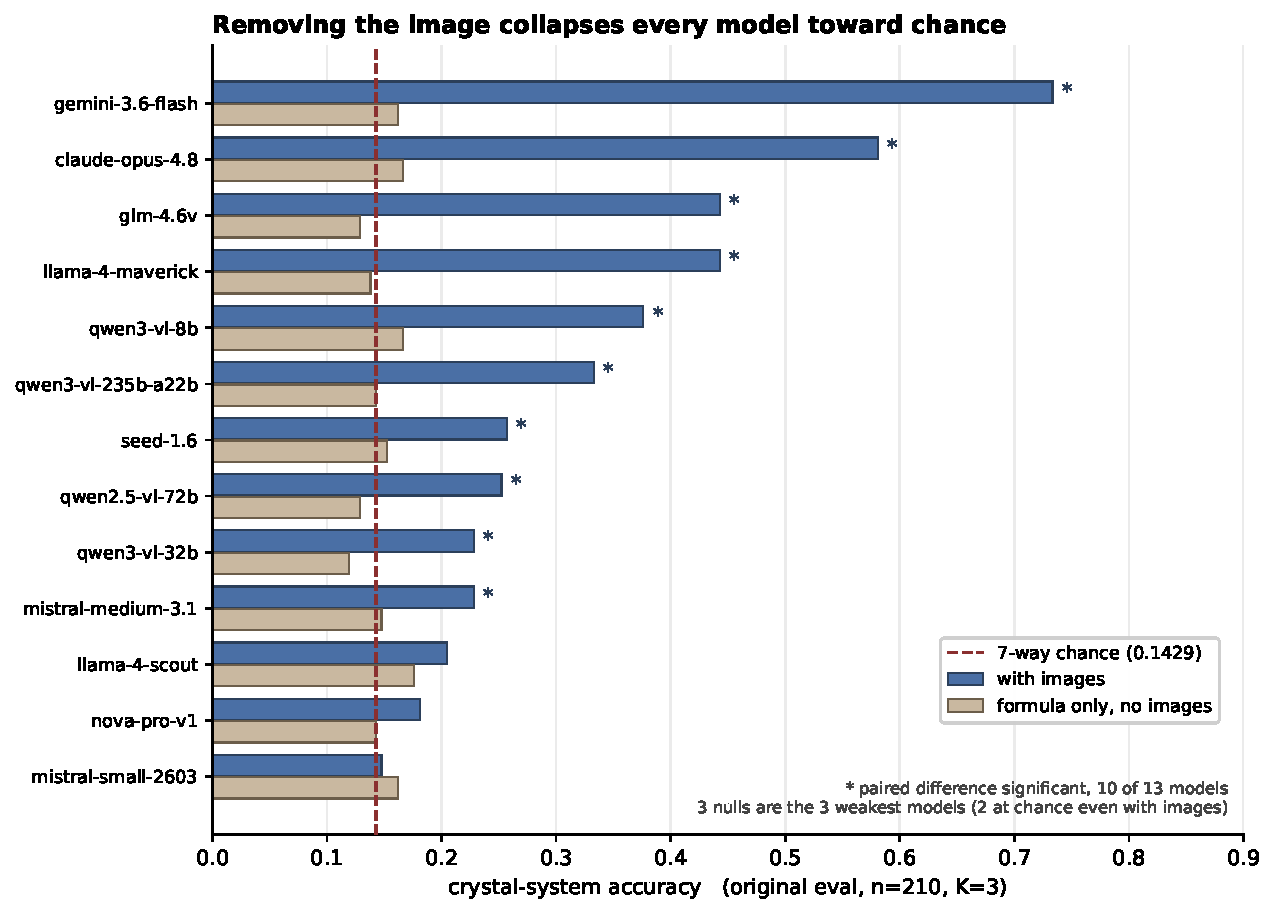
\includegraphics[width=0.8\linewidth]{figures/noimage.pdf}
\caption{Image-removal control: each model answered the identical prompt with the five renders and with the
chemical formula alone, paired per structure (original sample, $n=210$, $K=3$, 13 scored of 16 attempted).
Stars mark models whose paired difference is significant; the dashed line is seven-way chance.}
\label{fig:noimage}
\end{figure}

\paragraph{The strongest model arm, and what is not claimed for it.}
The 0.6905 figure is a supervised-then-GRPO arm on \texttt{Qwen/Qwen3-VL-8B-Instruct}, reported as a
single-seed point estimate at $K{=}8$; the same adapter gives $139/210 = 0.6619$ at $K{=}3$. It sits inside
the reference arm's across-seed spread ($0.590 / 0.567 / 0.686$), exceeding that arm's best seed by one
structure at $K{=}8$ and trailing it by five at $K{=}3$, so \emph{we make no claim that this arm improves
on the reference arm}. It is used only as the model side of the ceiling-to-model gap (200 against 145,
discordance $61{:}6$, $p = 1.5\times10^{-12}$), which survives any seed in the observed spread. The
three-seed extension was cut; its record and the quantitative argument for the cut are in the
supplementary.
